\documentclass[a4paper,12pt]{article}
%%%%%%%%%%%%%%%%%%%%%%%%%%%%%%%%%%%%%%%%%%%%%%%%%%%%%%%%%%%%%%%%%%%%%%%%%%%%%%%%%%%%%%%%%%%%%%%%%%%%%%%%%%%%%%%%%%%%%%%%%%%%%%%%%%%%%%%%%%%%%%%%%%%%%%%%%%%%%%%%%%%%%%%%%%%%%%%%%%%%%%%%%%%%%%%%%%%%%%%%%%%%%%%%%%%%%%%%%%%%%%%%%%%%%%%%%%%%%%%%%%%%%%%%%%%%
\usepackage{eurosym}
\usepackage{vmargin}
\usepackage{amsmath}
\usepackage{fancyhdr}
\usepackage{listings}
\usepackage{framed}
\usepackage{graphics}
\usepackage{epsfig}
\usepackage{subfigure}
\usepackage{fancyhdr}

\setcounter{MaxMatrixCols}{10}
%TCIDATA{OutputFilter=LATEX.DLL}
%TCIDATA{Version=5.00.0.2570}
%TCIDATA{<META NAME="SaveForMode" CONTENT="1">}
%TCIDATA{LastRevised=Wednesday, February 23, 2011 13:24:34}
%TCIDATA{<META NAME="GraphicsSave" CONTENT="32">}
%TCIDATA{Language=American English}

\pagestyle{fancy}
\setmarginsrb{20mm}{0mm}{20mm}{25mm}{12mm}{11mm}{0mm}{11mm}
\lhead{MA4704} \rhead{Mr. Kevin O'Brien}
\chead{Technological Mathematics 4}
%\input{tcilatex}

\begin{document}

\tableofcontents

\section*{Sample Papers}
\begin{itemize}
\item Current Version : Friday 19th April 2013
\item End of year exam paper is worth 70\% of module grade.
\item There will be five questions. You must attempt four.
\item This sample paper will have multiple variants for each of the five questions.
\end{itemize}
\newpage

%\section*{Attempt 4 questions from 5}
%----------------------------------------------------------------------------------%
\subsection*{Q.1 Descriptive Statistics (Variant 1)}
\subsubsection*{Part A} %10 MARKS
Data on the durations (measured in months) were collected for a random sample of product development projects.
The durations for these development projects were collected and tabulated as follows:

\begin{table}[ht]
\begin{center}
\begin{tabular}{|rrrrrrrr|}

\hline
12 & 11 & 20 & 19 & 18 & 9 & 16 & 15 \\
\hline
\end{tabular}
\end{center}
\end{table}
\vspace{-0.5cm}


\begin{itemize}
\item[i.](1 Mark) Calculate the mean of the project durations.
\item[ii.](2 Marks) Calculate the variance for this sample.
\item[iii.](1 Mark) Calculate the standard deviation for this sample.
\end{itemize}

\subsubsection*{Part B} %10 MARKS
A telecommunications company has two servers from different suppliers. The Operations Director randomly selected 9 months from the previous year's figures.  The down time figures for each server is as follows (down time per month in hours)

\begin{center}
\begin{tabular}{|c|c|c|}
  \hline
	&Server 1&	Server 2\\\hline
1	&5.3	&5.4\\
2	&5.4	&5.5\\
3	&5.5	&6.1\\
4	&5.2	&5.0\\
5	&5.1	&5.1\\
6	&5.6	&5.2\\
7	&5.4	&5.3\\
8	&5.5	&5.4\\
9	&5.6	&5.9\\
10  &5.6    &5.2\\
  \hline
\end{tabular}
\end{center}

\begin{itemize}
\item[i.](8 Marks) You are required to construct a box plot for each server's output and to comment on the salient features of each plot.  Is there evidence from the box plots to reject the hypothesis that there is no difference in the down time between the two servers?  Use the box plot to justify your comments. 							 \item[ii.](2 Marks)Compare and contrast the Mean and the Median as measures of location
\end{itemize}


%----------------------------------------------------------------------------------%
\newpage
\subsection*{Q.1 Descriptive Statistics (Variant 2)}
\subsubsection*{Part A} %28 MARKS
The exam results for a class of 40 students are tabulated below.
\begin{table}[ht]
\begin{center}
\begin{tabular}{|rrrrrrrrrr|}
\hline
 20 & 36 & 37 & 37 & 41 & 43 & 44 & 44 & 44 & 45 \\
 49 & 50 & 51 & 52 & 52 & 52 & 52 & 53 & 53 & 53 \\
 54 & 55 & 55 & 57 & 57 & 59 & 59 & 59 & 62 & 62 \\
 65 & 66 & 67 & 70 & 71 & 74 & 86 & 87 & 89 & 98 \\

\hline
\end{tabular}
\end{center}
\end{table}
\vspace{-0.5cm}
\begin{itemize}
\item[i.] (4 Marks) Summarize the data in the above table using a relative frequency table and a cumulative relative frequency table. Use 6 class intervals, with 11 as the lower limit of the first interval.
\item[ii.] (5 Marks) Draw a histogram for the above data. Comment on the shape of the histogram. Based on the shape of the histogram, what is the best measure of centrality and variability?
\item[iii.] (7 Marks) Construct a box plot for the above data. Clearly demonstrate how all of the necessary values were computed.
\end{itemize}

\vspace{0.25cm}
\subsubsection*{Part B} %28 MARKS
Consider the following data set of seven numbers:

\begin{center}
\textbf{\texttt{29 14 17 30 19 25 13}}
\end{center}
% 4 Marks

\noindent For this sample, compute the following descriptive statistics:
\begin{itemize}
%\item[a.] (1 Mark) The median,
\item[i.] (1 Mark) The mean,
\item[ii.] (2 Mark) The variance,
\item[iii.] (1 Mark) The standard deviation.
\end{itemize}
(End of Question)
%----------------------------------------------------------------------------------%
\newpage
\subsection*{Q.1 Descriptive Statistics (Variant 3)}
\subsubsection*{Part A} %10 MARKS
The mass of 30 individuals (in kg) was observed. The results are given below
\begin{center}

\begin{tabular}{|c c c c c c c c c c|}
  \hline
37&44&48&51&53&56&58&60&62&63\\
65&67&69&70&72&74&76&77&79&81\\
83&86&88&91&94&97&101&106&113&127\\
  \hline
\end{tabular}

\end{center}
\begin{itemize}
\item[i.](6 Marks) Construct a relative frequency and cumulative relative frequency table for this data set.
\item[i.](6 Marks)Draw a histogram for these data. Comment on the shape of the histogram.
\item[ii.](8 Marks) Draw the boxplot for this sample.
\end{itemize}
(End of Question)
%------------------------------------------------------------------------------------------------ %
\newpage
\subsection*{Q.2 Probability (Variant 1)}

\subsubsection*{Part A}
 The probability distribution of discrete random variable $X$ is tabulated below. There are 5 possible outcomes of $X$, i.e. 1, 2, 3, 5 ,10 and 20.
\begin{center}
\begin{tabular}{|c||c|c|c|c|c|}
\hline
$x_i$  & 1 & 2 & 5 & 10 & 20 \\\hline
$P(x_i)$ &  0.10 & 0.25 & 0.30& 0.20 &0.15\\

\hline
\end{tabular}
\end{center}

\begin{itemize}
\item[i.] (3 Marks) Determine the expected value $E(X)$.
\item[ii.] (3 Marks) Evaluate $E(X^2)$.
\item[iii.] (2 Marks) Compute the variance of random variable $X$.
\end{itemize}


\subsubsection*{Part B}
An electronics assembly subcontractor receives its entire supply of resistors from two suppliers. Company A provides 70\% of the subcontractor's resistors ,while company B supplies the remainder. The additional information has also been made available.
\begin{itemize}
\item 2\% of the resistors provided by company A failed the final test,
\item 3\% of company B's resistors also fail final test.
\end{itemize}
\noindent Answer the following questions:
\begin{itemize}
\item[i.](3 Marks) What is the probability that a resistor fails the final test?
\item[ii.](3 Marks)  What is the probability that a resistor fails the final test given that the resistor in question came from company A?
%\item[iii.](2 marks) What is the probability that a resistor that fails final test was supplied by company A?
\end{itemize}


%------------------------------------------------------------------------------------------------ %
\newpage
\subsection*{Q.2 Probability (Variant 2)}
\subsubsection*{Part A}
The probability distribute of discrete random variable $X$ is tabulated below. There are 5 possible outcome of $X$, i.e. 1, 2, 4, 6 and 8.
\begin{center}
\begin{tabular}{|c||c|c|c|c|c|}
\hline
$x_i$  & 1 & 2 & 4 & 6 & 8  \\\hline
$p(x_i)$ & 0.50 & 0.15 & 0.20 & 0.05 & 0.10 \\
\hline
\end{tabular}
\end{center}

\begin{itemize}
%\item[a.] (1 Mark) Compute the value of $k$.
\item[i.] (2 Mark) What is the expected value of X?
%\item[c.] (1 Mark) Compute the value of $E(X^2)$
\item[ii.] (2 Mark) Given that $E(X^2) = 12.5$, compute the variance of $X$.
\end{itemize}


\subsubsection*{Part B}
On completion of a programming project, four programmers from a team submit a collection of subroutines to an acceptance group. The following table shows the percentage of subroutines each programmer submitted and the probability that a subroutine submitted by each programmer will pass the certification test based on historical data.


\begin{center}
\begin{tabular}{|c||c|c|c|c|}
\hline
Programmer	&A	&B	&C	&D\\
Proportion of subroutines submitted &	0.10&	0.20&	0.30&	0.40\\
Probability of acceptance	&0.55	&0.60	&0.95&	0.75\\
\hline
\end{tabular}
\end{center}


\begin{itemize}
\item[i.](3 Marks) What is the proportion of subroutines that pass the acceptance test?
\item[ii.](3 Marks) After the acceptance tests are completed, one of the subroutines is selected at random and found to have passed the test. What is the probability that it was written by Programmer A?
\end{itemize}

\subsubsection*{Part c} % 6 Marks
A doctor treating a patient issues a prescription for antibiotics and provides for two repeat prescriptions. The probability that the infection will be cleared by the first prescription is $p_1$ =0.6.
The probability that successive treatments are successful, given that previous prescriptions were not successful are $p_2$ = 0.5, $p_3$ = 0.4. Calculate the probability that:

\begin{itemize}
\item[i.](2 Marks) a patient will require the third prescription,
\item[ii.](2 Marks) the patient is still infected after the third prescription,
\item[iii.](2 Marks) the patient is cured by the second prescription, given that the patient is eventually cured.
\end{itemize}

%------------------------------------------------------------------------------------------------ %
\newpage
%Question 3
%A) Normal Distribution 8 Marks
%B) Binomial Distribution - Not Actioned
%C) Poisson 6 Marks
%D) Exponential 6 Marks

% Almost Ready

\subsection*{Q.3 Probability Distributions (Variant 1)}

\subsubsection*{Part A} % Exponential %6 MARKS
Suppose that a student is taking a multiple-choice exam in which each question has four choices.
Suppose that she has no knowledge of the correct answer to any of the questions. Furthermore suppose that she selects one of the possible choices at random as her answer.
\begin{itemize}
\item [i.](2 Marks) If there are five multiple-choice questions on the exam, what is the probability that she will answer four questions correctly.
\item [ii.](2 Marks) What is the probability that she will answer none of the questions correctly?
\item [iii.](2 Marks) What is the probability that she will answer at least two questions correctly?
\end{itemize}

\subsubsection*{Part B} % Exponential %6 MARKS
A power supply unit for a computer component is assumed to follow an exponential distribution with a mean life of 1,400 hours.  What is the probability that the component will:
\begin{itemize}
\item [i.](2 Marks)	fail in the first 700 hours?
\item [ii.](2 Marks) survive more than 1,750 hours?
\item [iii.](2 Marks) last between 1,050 hours and 1,750 hours?
\end{itemize}



\subsubsection*{Part C} % Normal %6 MARKS
Assume that the diameter of a critical component is normally distributed with a Mean of 50mm and a Standard Deviation of 2mm.

NB 	You must draw a rough sketch of the normal curve and estimate the approximate probability of the following measurements occurring on an individual component.
\begin{itemize}
\item [i.](2 Marks)	Between 50 and 51.2mm
\item [ii.](2 Marks) Less than 48.5 mm
\item [iii.](2 Marks) Between 48.2 and 101.6 mm
\end{itemize}

Use the normal tables to get the exact probabilities for the above.
						

%---------------------------------------------------------------------------------------------%
\newpage
\subsection*{Q.3 Probability Distributions (Variant 2)}



\subsubsection*{Part A}% Poisson %6 MARKS
Telephone calls arrive at a switchboard at a rate of 30 per hour.  Assume that the switchboard operators take 2 minutes to deal with a customer query. Calculate the following:

\begin{itemize}
\item [i.](2 Marks)	The probability of 2 or more calls arriving in any 4 minute period,
\item [ii.](2 Marks) The probability of no phone calls arriving in a 4 minute period,
\item [iii.](2 Marks) The probability of exactly three phone call arriving in a 10 minute period.
%\item [iv.]	The average and standard deviation of the number of phone calls arriving in a 2 minute period.

\end{itemize}
\subsubsection*{Part B} %NORMAL %8 MARKS
Assume that the length of injected moulded plastic components are normally distributed with a mean of 12.5mm and a standard deviation of 2.5mm.  Calculate the corresponding probability for the following measurements occurring on an individual component.

\begin{itemize}
\item [i.](2 Marks)	Between 12.5 and 15mms,
\item [ii.](2 Marks) Less than 10 mms,
\item [iii.](2 Marks) Between 12 and 15 mms,
\item [iv.](2 Marks) Less than 10.3 mms.
\end{itemize}
\noindent Illustrate each of your answers with a sketch.

\subsubsection*{Part C} %Binomial
It is estimated by a particular bank that 25\% of credit card customers pay only the minimum amount due on their monthly credit card bill and do not pay the total amount due. 50 credit card customers are randomly selected.
\begin{enumerate}
\item (3 marks)	What is the probability that 9 or more of the selected customers pay only the minimum amount due?
\item (3 marks) What is the probability that less than 6 of the selected customers pay only the minimum amount due?
\item (3 marks)	What is the probability that more than 5 but less than 10 of the selected customers pay only the minimum amount due?
\end{enumerate}



%---------------------------------------------------------------------------------------------%
\newpage
\subsection*{Q.3 Probability Distributions (Variant 3)}
\subsubsection*{Part A} %Poisson %8 MARKS
Flaws occur in an LCD display at the rate of 0.5 per square mm.  Calculate the probability that:

\begin{itemize}
\item [i.](2 Marks)	exactly 2 flaws will occur in a square mm section,
\item [ii.](2 Marks) exactly 3 flaws will occur in a 5 square mm section,
\item [iii.](2 Marks) 5 or more flaws will occur in a 10 square mm section.
\end{itemize}

\subsubsection*{Part B} %Exponential
The average lifespan of a PC monitor is 6 years. You may assume that the lifespan of monitors follows an exponential probability distribution.
    \begin{enumerate}
    \item (2 marks) What is the probability that the lifespan of the monitor will be at least 5 years?
    \item (2 marks) What is the probability that the lifespan of the monitor will not exceed 4 years?
    \item (2 marks) What is the probability of the lifespan being between 5 years and 7 years?
    \end{enumerate}

\subsubsection*{Part C} % Normal
A machine is used to package bags of potato chips.  Records of the packaging machine indicate that its fill weights are normally distributed with a mean of 455 grams per bag and a standard deviation of 10 grams.

    \begin{enumerate}
    \item (3 marks) What proportion of bags filled by this machine will contain more than 470 grams in the long run?
    \item (3 marks)	What proportion of bags filled by this machine will contain less than 445 grams in the long run?
    \item (2 marks)	What proportion of bags filled by this machine will be between 465 grams and 475 grams in the long run?
    \end{enumerate}
%------------------------------------------------------------------------------------------------ %
\newpage

% Question 4  Hypothesis Testing  + Confidence Intervals
% Good Shape

\subsection*{Q4. Inference Procedures (Variant 1)}

\subsubsection*{Part A} %4 Marks
\begin{itemize}
\item[i.](2 Marks) In the context of hypothesis testing, explain what a p-value is, and how it is used. Support your answer with a simple example.
\item[ii.](2 Marks) What is meant by Type I error and Type II error?
\end{itemize}
\subsubsection*{Part B} %3 Marks
A well-known polling company estimates that $57\%$ of Irish voters support a new constitutional amendment. 800 people were randomly surveyed and asked about their voting preferences. 482 of the 800 people responded positively to the amendment. You are required to:

\begin{itemize}
\item [i.](1 Mark) Obtain a point estimate of the proportion of people supporting the constitutional amendment.
\item [ii.](2 Marks) Construct a 95\% confidence interval for the proportion of people in favour of the constitutional amendment.
\end{itemize}

\subsubsection*{Part C} %4 Marks
The standard deviations of data sets \texttt{X} and \texttt{Y} are 10 and 9 respectively. An inference procedure was carried out to assess whether or not \texttt{X} and \texttt{Y} can be assumed to have equal variance.
\begin{itemize}
\item[i.](1 Mark) Formally state the null and alternative hypothesis.
\item[ii.](1 Mark) The Test Statistic has been omitted from the computer code output. Compute the value of the Test Statistic.
\item[iii.](2 Marks) What is your conclusion for this procedure? Justify your answer.
%\item[iv.] (1 Marks) Explain how a conclusion for this procedure can be based on the $95\%$ confidence interval.
\end{itemize}

%---- R code for Variance Test ----%
%---- Dummy Code Included                   ----%
\begin{framed}
\begin{verbatim}
        F test to compare two variances

data:  X and Y
F = ......, num df = 13, denom df = 11, p-value = 0.7349
alternative hypothesis: true ratio of variances is not equal to 1
95 percent confidence interval:
 0.3639938 3.9475262
sample estimates:
ratio of variances
          .......
\end{verbatim}
\end{framed}

\subsubsection*{Part D} %9 Marks
Two samples of students are randomly selected from two IT training companies; Echelon and Deltatech. The mean and the standard deviation of the number of marks obtained in a well known IT competency exam by both sets of students are described below:\\

\begin{center}
\begin{tabular}{|c|c|c|c|}

  \hline
  % after \\: \hline or \cline{col1-col2} \cline{col3-col4} ...
	&Number&	Mean&	Std. Dev.\\ \hline
DeltaTech	&14	&24	&10\\
Echelon	&12	&22.5	&9\\
  \hline
\end{tabular}
\end{center}

%Calculate a 95\% confidence interval for the difference between the mean number of marks obtained by males and females in the population of school leavers as a whole.
%(7 marks)

Test the hypothesis that Echelon students and DeltaTech students, on average, obtain the same mark in the IT certification exam. Use a significance level of $5\%$. You may assume that any required assumptions have been validated.
% State your hypotheses clearly. What is the significance level of this test?
\bigskip

\begin{itemize}
\item[i.](2 Marks) Formally state the null and alternative hypotheses.
\item[ii.](3 Marks) Compute the Test Statistic.
\item[iii.](2 Marks) State the appropriate Critical Value for this hypothesis test.
\item[iv.](2 Marks) Discuss your conclusion to this test, supporting your statement with reference to appropriate values.
\end{itemize}

%------------------------------------------------------------------------------------------------ %
\newpage

% Question 4  Hypothesis Testing  + Confidence Intervals
% Good Shape

\subsection*{Q4. Inference Procedures (Variant 2)}

\subsubsection*{Part A} %4 Marks
\begin{itemize}
\item[i.](2 Marks) In the context of hypothesis testing, explain what a p-value is, and how it is used. Support your answer with a simple example.
\item[ii.](2 Marks) What is meant by Type I error and Type II error?
\end{itemize}

\subsubsection*{Part B} %4 Marks
\noindent The mean and the standard deviation of the number of marks obtained in the biology leaving certificate exam by randomly selected male and female pupils are described below:\\

\begin{center}
\begin{tabular}{|c|c|c|c|}

  \hline
  % after \\: \hline or \cline{col1-col2} \cline{col3-col4} ...
	&Number&	Mean&	Std. Dev.\\ \hline
Male	&10	&57	&12\\
Female	&12	&61	&11\\
  \hline
\end{tabular}
\end{center}

%Calculate a 95\% confidence interval for the difference between the mean number of marks obtained by males and females in the population of school leavers as a whole.
%(7 marks)

Test the hypothesis that males and females on average obtain the same mark in the biology leaving certificate exam. Use a significance level of $5\%$. You may assume that all required assumptions have been validated.\\% State your hypotheses clearly. What is the significance level of this test?
\bigskip
\begin{itemize}
\item[i.](2 Marks) Formally state the null and alternative hypotheses.
\item[ii.](3 Marks) Compute the Test Statistic.
\item[iii.](2 Marks) State the appropriate Critical Value for this hypothesis test.
\item[iv.](2 Marks) Discuss your conclusion to this test, supporting your statement with reference to appropriate values.
\end{itemize}

\subsubsection*{Part C} %4 Marks
Consider the following inference procedure performed on data set $X$.
\begin{center}
\begin{verbatim}
> shapiro.test(X)

        Shapiro-Wilk normality test

data:  X
W = 0.9619, p-value = 0.6671

\end{verbatim}
\end{center}


\begin{itemize}
\item[i.] (1 Mark) Describe what is the purpose of this procedure.
\item[ii.] (2 Marks) What is the null and alternative hypothesis?
\item[iii.] (1 Mark) Write the conclusion that follows from it.
\end{itemize}



%-------------------------------------------------------------------------------------------------- %

\newpage
\subsection*{Q4. Inference Procedures (Variant 3)}
\subsubsection*{Part A} %4 Marks
The strength of dosage of a plant growth enhancement chemical is often measured by the proportion of plants that grow faster. A particular dosage of the chemical is fed to 115 plants of these plants, 94 actually show faster growth.

 \begin{itemize}
\item[i.] Calculate a point estimate $\hat{p}$ for the proportion of plants that grow faster due to the dosage. 									 
\item[ii.]  What is the standard error of the estimate? 			
\item[iii.] Find a 95\% confidence interval for p. 					
\item[iv.] What size sample is required to give the estimate in (c) to within $\pm1\%$. 	
\item[v.] Carry out a testing procedure to investigate the claim that the chemical is 90\%   effective. 								 \end{itemize}

\subsubsection*{Part B} %4 Marks
The data set \texttt{Y} is both assumed to be normally distributed. A graphical procedure was carried out to assess whether or not this assumption of normality is valid for data set \texttt{Y}. Consider the Q-Q plot in the figure below.

\begin{center}
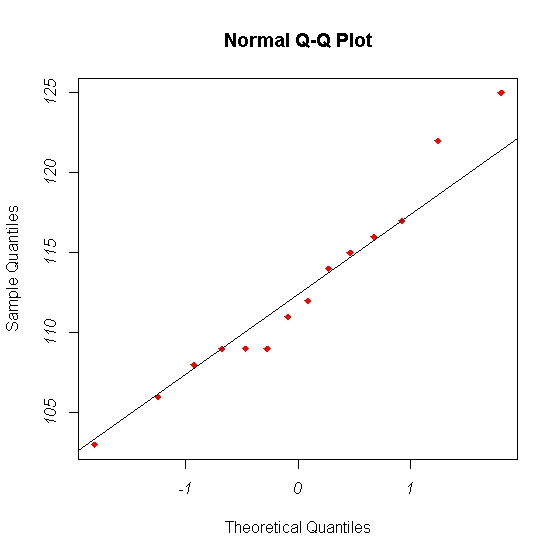
\includegraphics[scale=0.55]{Q5examQQplot}
\end{center}

\begin{itemize}
\item[i.] (2 marks) Provide a brief description on how to interpret this plot.
\item[ii.] (1 marks) What is your conclusion for this procedure? Justify your answer.
\end{itemize}



\subsubsection*{Part C} %4 Marks
 \begin{tabular}{|cccc|}
   \hline
   % after \\: \hline or \cline{col1-col2} \cline{col3-col4} ...
6.98 &8.49 &7.97& 6.64\\
8.80 &8.48 &5.94& 6.94\\
6.89 &7.47 &7.32& 4.01\\
   \hline
 \end{tabular}

\begin{center}
\begin{verbatim}
> grubbs.test(x, two.sided=T)

        Grubbs test for one outlier

data:  x
G = 2.4093, U = 0.4243, p-value = 0.05069
alternative hypothesis: lowest value 4.01 is an outlier
\end{verbatim}
\end{center}
\begin{itemize}
\item[i.] (2 marks) Describe what is the purpose of this procedure.
\item[ii.] (2 marks) Write the conclusion that follows from it.
\end{itemize}
%-------------------------------------------------------------------------------------------------- %

\newpage
\subsection*{Q4. Inference Procedures (Variant 4)}
\subsubsection*{Part A} %4 Marks
\begin{itemize}
\item[i.](2 Marks) In the context of hypothesis testing, explain what a p-value is, and how it is used. Support your answer with a simple example.
\item[ii.](2 Marks) What is meant by Type I error and Type II error?
\end{itemize}
\subsubsection*{Part B} %3 Marks
A well-known polling company estimates that $57\%$ of Irish voters support a new constitutional amendment. 800 people were randomly surveyed and asked about their voting preferences. 482 of the 800 people responded positively to the amendment. You are required to:

\begin{itemize}
\item [i.](1 Mark) Obtain a point estimate of the proportion of people supporting the constitutional amendment.
\item [ii.](2 Marks) Construct a 95\% confidence interval for the proportion of people in favour of the constitutional amendment.
\end{itemize}


\subsubsection*{Part C} %4 Marks
A graphical procedure was carried out to assess whether or not this assumption of normality is valid for data set \texttt{Y}. Consider the Q-Q plot in the figure below.

\begin{center}
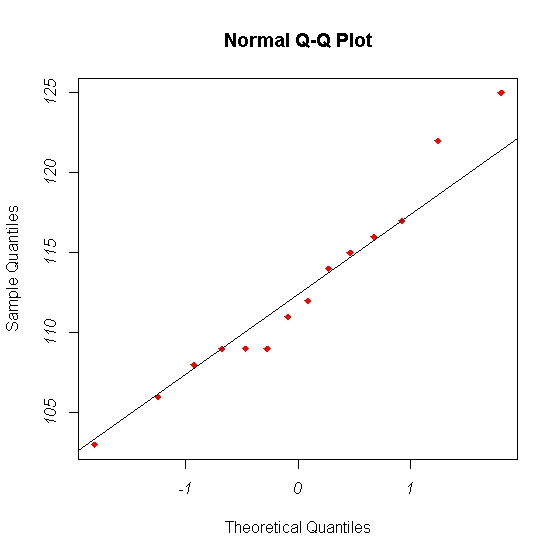
\includegraphics[scale=0.55]{Q5examQQplot}
\end{center}

\begin{itemize}
\item[i.] (2 marks) Provide a brief description on how to interpret this plot.
\item[ii.] (1 marks) What is your conclusion for this procedure? Justify your answer.
\end{itemize}
%\end{itemize}
%-------------------------------------------------------------------------------------------------- %
\newpage
\subsection*{Q5. Correlation and Linear Regression (Variant 1)}
A fire insurance company wants to relate the amount of fire damage in major residential fires to the distance between the residence and the nearest fire station. The study is to be conducted in a large suburb of a major city; a sample of 15 recent fires in this suburb is selected. The amount of damage (thousands of pounds) and the distance (in Kilometers) between the fire and the nearest station are recorded for each fire.

\begin{center}
\begin{tabular}{|c|c|c|c|c|c|}
  \hline
Incident	&	Distance (X) 	&	Fire Damage (Y)   	&	Incident	&	Distance (X) 	& Fire Damage (Y)   		 \\
1	&	3.4	&	21	&	9	&	2.6	&	15	\\
2	&	1.8	&	13	&	10	&	4.3	&	26	\\
3	&	4.6	&	26	&	11	&	2.1	&	19	\\
4	&	2.3	&	18	&	12	&	1.1	&	12	\\
5	&	3.1	&	23	&	13	&	6.1	&	38	\\
6	&	5.5	&	31	&	14	&	4.8	&	31	\\
7	&	0.7	&	9	&	15	&	3.8	&	21	\\
8	&	3	&	17	&		&		&		\\

  \hline
\end{tabular}



\begin{tabular}{lll}
  $\sum X = 49.2$ & $\sum Y = 320$ & $\sum XY = 1219.2$ \\
  $\sum X^2 = 196.16$ & $\sum Y^2 = 7722$ &  \\
 \end{tabular}
 \end{center}


\begin{itemize}
\item[i.](5 Marks) Illustrate the data in a scatter diagram.
\item[ii.](5 Marks) Compute the value of the correlation coefficient.
\item[iii.](5 Marks) Find the equation of the regression line and plot the regression line on the scatter  diagram. Interpret the equation. 	
\item[v.](5 Marks) Using a significance level of $\alpha = 0.05$, test the claim that there is no linear correlation between distance and fire damage. 		
\end{itemize}

%-------------------------------------------------------------------------------------------------- %
\newpage
\subsection*{Q5. Correlation and Linear Regression (Variant 2)}
% Correlation and Simple Linear Regression
% Non Parametric Procedures

A wood scientist wanted to establish if there was a relationship between the adhesive strength of laminated wood and the dwell time in press machine. A random sample of 9 different times and their corresponding adhesive strengths in pounds per square inch (PSI) were recorded as follows:

\begin{center}
\begin{tabular}{|c|c|c|}

  \hline
Sample &Time (Mins) & Pull Strength (PSI) \\
 & (X)  &  (Y)\\ \hline
1& 5.0& 3.5 \\
2& 4.8& 3.3\\
3& 5.6& 3.9\\
4& 4.3& 2.7\\
5& 4.2& 3.2\\
6& 5.4& 4.1\\
7& 5.5& 4.3\\
8& 4.0& 2.8\\
9& 4.7& 3.7\\
  \hline
\end{tabular}
\bigskip

\begin{tabular}{lll}
  $\sum X = 43.5$ & $\sum Y = 31.5$ & $\sum XY = 154.61$ \\
  $\sum X^2 = 213.03$ & $\sum Y^2 = 112.71$ &  \\
 \end{tabular}
 \end{center}
\begin{itemize}
\item[i.](5 Marks) Draw a scatter-plot and comment on its features.
\item[ii.](5 Marks) Calculate the correlation coefficient. Interpret your answer.
\item[iii.](5 Marks) Calculate the equation of the least squares regression line and interpret the value of the slope.
\item[iv.](3 Marks) Using this regression model, estimate the adhesive strength for a piece of wood that has been in the press machine for 7 minutes.
\item[v.](2 Marks) Is such an estimate reliable? Briefly explain why.
\end{itemize}
%-------------------------------------------------------------------------------------------------- %
\newpage
\subsection*{Q5. Correlation and Linear Regression (Variant 3)}
% Correlation and Simple Linear Regression
% Non Parametric Procedures
The following scatter-plot illustrates the relationship between the period of a pendulum in seconds and its length in metres (for 13 different lengths of the pendulum).

\begin{center}
\includegraphics[scale=0.55]{Q5examScatter}
\end{center}
Use the following statistics to answer the following questions
%
%SX,Y = ;   SX,X = 3.629;     SY,Y = 2.700
%? xi = 11.3;    ? yi = 17.827
\begin{center}
\begin{tabular}{lll}
  $\sum X = 43.5$ & $\sum Y = 31.5$ & $\sum XY = 3.068$ \\
  $\sum X^2 = 213.03$ & $\sum Y^2 = 112.71$ &  \\
 \end{tabular}
 \end{center}
i)	Calculate the equation of the least squares regression line and interpret the value of the slope.
(5 marks)
ii)	Using this regression model, estimate the period of a pendulum of length 4m.
(2 marks)
iii)	Briefly explain why this estimate is not reliable.
(2 marks)

%-------------------------------------------------------------------------------------------------- % \newpage
\newpage
\section*{Formulae}
%-------------------------------------------------%
\subsection*{Descriptive Statistics}
\begin{itemize}
\item Sample Variance
\begin{equation*}
s^2 = \frac{\sum (x-\bar{x})^2}{n-1}
\end{equation*}
\end{itemize}
%-------------------------------------------------%
\subsection*{Probability}
\begin{itemize}

\item Conditional probability:
\begin{equation*}
P(B|A)=\frac{P\left( A\text{ and }B\right) }{P\left( A\right) }.
\end{equation*}


\item Bayes' Theorem:
\begin{equation*}
P(B|A)=\frac{P\left(A|B\right) \times P(B) }{P\left( A\right) }.
\end{equation*}





\item Binomial probability distribution:
\begin{equation*}
P(X = k) = ^{n}C_{k} \times p^{k} \times \left( 1-p\right) ^{n-k}\qquad \left( \text{where  }
^{n}C_{k} =\frac{n!}{k!\left(n-k\right) !}. \right)
\end{equation*}

\item Poisson probability distribution:
\begin{equation*}
P(X = k) =\frac{m^{k}\mathrm{e}^{-m}}{k!}.
\end{equation*}

\item Exponential probability distribution:
\begin{equation*}
P(X \leq k) = \begin{cases}
1-e^{- k/\mu}, & k \ge 0, \\
0, & k < 0.
\end{cases}\qquad \left( \text{where  }
\mu = {1\over \lambda}\right)
\end{equation*}
\end{itemize}



\subsection*{Confidence Intervals}
{\bf One sample}
\begin{eqnarray*} S.E.(\bar{X})&=&\frac{\sigma}{\sqrt{n}}.\\\\
S.E.(\hat{P})&=&\sqrt{\frac{\hat{p}\times(100-\hat{p})}{n}}.\\
\end{eqnarray*}
{\bf Two samples}
\begin{eqnarray*}
S.E.(\bar{X}_1-\bar{X}_2)&=&\sqrt{\frac{\sigma^2_1}{n_1}+\frac{\sigma_2^2}{n_2}}.\\\\
S.E.(\hat{P_1}-\hat{P_2})&=&\sqrt{\frac{\hat{p}_1\times(100-\hat{p}_1)}{n_1}+\frac{\hat{p}_2\times(100-\hat{p}_2)}{n_2}}.\\\\
\end{eqnarray*}
\subsection*{Hypothesis tests}
{\bf One sample}
\begin{eqnarray*}
S.E.(\bar{X})&=&\frac{\sigma}{\sqrt{n}}.\\\\
S.E.(\pi)&=&\sqrt{\frac{\pi\times(100-\pi)}{n}}
\end{eqnarray*}
{\bf Two large independent samples}
\begin{eqnarray*}
S.E.(\bar{X}_1-\bar{X}_2)&=&\sqrt{\frac{\sigma^2_1}{n_1}+\frac{\sigma_2^2}{n_2}}.\\\\
S.E.(\hat{P_1}-\hat{P_2})&=&\sqrt{\left(\bar{p}\times(100-\bar{p})\right)\left(\frac{1}{n_1}+\frac{1}{n_2}\right)}.\\
\end{eqnarray*}
{\bf Two small independent samples}
\begin{eqnarray*}
S.E.(\bar{X}_1-\bar{X}_2)&=&\sqrt{s_p^2\left(\frac{1}{n_1}+\frac{1}{n_2}\right)}.\\\\
s_p^2&=&\frac{s_1^2(n_1-1)+s_2^2(n_2-1)}{n_1+n_2-2}.\\
\end{eqnarray*}
{\bf Paired sample}
\begin{eqnarray*}
S.E.(\bar{d})&=&\frac{s_d}{\sqrt{n}}.\\\\
\end{eqnarray*}
{\bf Standard Deviation of case-wise differences (computational formula)}
\begin{eqnarray*}
s_d = \sqrt{ {\sum d_i^2 - n\bar{d}^2 \over n-1}}.\\\\
\end{eqnarray*}


\noindent{\bf Regression estimates}

\begin{eqnarray*}
S_{XY} &=&
\sum x_iy_i - \frac{\sum x_i\sum y_i}{n}\\
S_{XX} &=&
\sum x_i^2 - \frac{(\sum x_i)^2}{n}\\
S_{YY} &=&
\sum y_i^2 - \frac{(\sum y_i)^2}{n}\\
\end{eqnarray*}
{\bf Slope Estimate}
\begin{eqnarray*}
b_1 = \frac{S_{XY}}{S_{XX}}
\end{eqnarray*}
{\bf Intercept Estimate}
\begin{eqnarray*}
 b_0 = \bar{y} -b_1\bar{x}
\end{eqnarray*}
{\bf Pearson's correlation coefficient}

\begin{eqnarray*}
r = \frac{S_{XY}}{\sqrt{S_{XX} \times S_{YY}}}
\end{eqnarray*}
{\bf Standard error of the Slope}
\begin{eqnarray*}
S.E.(b1) = \sqrt{\frac{s^2}{S_{XX}}}
\end{eqnarray*}

where $s^2 = \frac{SSE}{n-2}$
and SSE $= S_{YY} - b_1S_{XY}$
\end{document} 